\documentclass[a4paper,12pt]{article} 



%Добавляет возможность искать и копировать текст
\usepackage{cmap}

%Убирает пробел между названием таблицы/рисунка и самой таблицей/рисунком
\usepackage{caption}
\captionsetup[table]{skip= -0 cm}
\captionsetup[figure]{skip= -0 cm}

%Выравнивание названия таблиц по левому краю
%\usepackage[nooneline]{caption} 
%Размеры отступов 
\usepackage[left=20mm, top=20mm, right=20mm, bottom=20mm, footskip=10mm]{geometry}

%Рисунки
\usepackage{graphicx}
\usepackage{wrapfig} %обтекание элементов
\graphicspath{{graphs}{figures}}  % папки с картинками

%Русский язык в формулах
\usepackage{mathtext}

%  Русский язык
\usepackage[T2A]{fontenc}			
\usepackage[utf8]{inputenc}			
\usepackage[english,russian]{babel}	

%Готические буквы
\usepackage{amssymb}

% Математика
\usepackage{amsmath,amsfonts,amssymb,amsthm,mathtools} 
\usepackage{wasysym}

%Цветные подписи в таблице
\usepackage[table,xcdraw]{xcolor}

\usepackage{fancyhdr} % Колонтитулы
 	\pagestyle{fancy}
 	\renewcommand{\headrulewidth}{0.3mm}  % Толщина линейки, отчеркивающей верхний колонтитул
 	%\lfoot{Нижний левый}
 	%\rfoot{Нижний правый}
 	\rhead{Кафедра вакуумной электроники}
 	%\chead{Верхний в центре}
 	\lhead{Квадрупольный масс-анализатор}
 	% \cfoot{Нижний в центре} % По умолчанию здесь номер страницы
 	
 	
\begin{document} 

%Титульник 
\begin{titlepage}
	\begin{center}
		\large 	МИНИСТЕРСТВО ОБРАЗОВАНИЯ И НАУКИ РОССИЙСКОЙ ФЕДЕРАЦИИ\\
				МОСКОВСКИЙ ФИЗИКО-ТЕХНИЧЕСКИЙ ИНСТИТУТ \\
				(НАЦИОНАЛЬНЫЙ ИССЛЕДОВАТЕЛЬСКИЙ ИНСТИТУТ)\\ 
				ФИЗТЕХ-ШКОЛА ЭЛЕКТРОНИКИ, ФОТОНИКИ \\
				И МОЛЕКУЛЯРНОЙ ФИЗИКИ \\
		
		
		\vspace{4.0 cm}
		\LARGE{Кафедра вакуумной электроники \\ 
		Отчет \\
		по лабораторной работе} \\ 
		\LARGE \textbf{Масс спектроскопия остаточных газов} \\
		\LARGE \textbf{Квадрупольный масс-анализатор}
	\end{center}
	\vspace{3 cm} \large

	%Надо подумать как это нормально написать	
	\begin{flushleft}
		Работу выполнил \hspace{5.5cm}  \underline{\hspace{3cm}} А.И.Белостоцкий \\	
		\vspace{1cm}
		Работу принял, оценка \hspace{4.3cm} \underline{\hspace{3cm}}
	\end{flushleft}
	

	
	\vfill

	\begin{center}
	Долгопрудный, 2021 г.
	\end{center}
\end{titlepage}                                                                      

\section*{Цель работы}
\begin{itemize}
\item Ознакомиться с принципами работы квадрупольного масс-спектрометра
\item Исследовать масс-спектр остаточных газов
\item Напустить в вакуумный объем воздух и исследовать масс-спектр образовавшейся газовой смеси
\end{itemize}


\section*{Теоретические сведения}

\subsubsection*{Качественная картина параметрического резонанса}
	
\begin{wrapfigure}{l}{0.4\linewidth} 
	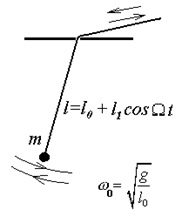
\includegraphics[width=\linewidth]{fig1}
	\caption{Параметрический резонанс \\ в математическом маятнике}				
\end{wrapfigure}

Уравнение движения маятника при фиксированной длине нити имеет вид (II закон Ньютона): $ml\frac{d^2\varphi}{dt^2}=-mgsin{\varphi}$(ф.1); ( угол на который нить отклоняетуся от положения равновесия ).  Если считать угол отклонения малым ( ;   х – горизонтальное отклонение от положения равновесия), то  получим из (ф.1)$ \frac{d^2x}{dt^2}=-\frac{g}{l_0}x, или: \frac{d^2x}{dt^2}=-\omega_0^2x$ (ф.2). При этом собственная частота колебаний маятника равна $\omega_0=\sqrt{\frac{g}{l_0}}$, а период колебаний $T=2\pi\sqrt{\frac{l_0}{g}}$ .

Пусть теперь длину нити маятника  изменяют во времени по периодическому закону $l(t)= l_0+ l_1cos\Omega t = l_0\left(1+\frac{l_1}{l_0}cos{\Omega}t\right)$ (рис. 1).   Тогда, если уменьшать длину нити в нижнем положении маятника, и увеличивать ее в крайних положениях,  то работа внешней силы за период оказывается положительной и амплитуда колебаний начнет возрастать. Иными словами, при параметрическом резонансе увеличение энергии колебаний  достигается  не периодической возмущающей силой, приложенной в направлении движения грузика m, а путем периодического изменения параметра системы, т.е. длины нити l. При этом период, с которым изменяется длина нити равен половине периода колебаний осциллятора. Соответственно частота такого возмущения $\Omega$ равна удвоенной частоте собственных колебаний . В теории параметрического резонанса периодическое изменение параметра колебательной системы называется накачкой, частота такого изменения W – частотой накачки, а отношение$\frac{l_1}{l_0}$ – глубиной накачки. Можно провести аналогичное рассмотрение для пружинного маятника (грузик на пружине), колебательного контура, состоящего из конденсатора и катушки индуктивности и т.п. Общее название для таких систем – осциллятор.  Все осцилляторы, независимо от их физической природы описываются одними и теми же дифференциальными уравнениями типа  (ф.2), отличающимися только обозначениями.  И во всех осцилляторах  можно наблюдать параметрическое возбуждение, если периодическим образом изменять  некоторый параметр осциллятора.
Параметрический резонанс в осцилляторах существенно отличается от обычного резонанса. Обычный (непараметрический) резонанс, возникает,  как хорошо  известно, в том случае, когда частота $\Omega$ периодической внешней возмущающей силы совпадает с собственной частотой   осциллятора. При этом поведение колебательной системы описывается неоднородным дифференциальным уравнением второго порядка с постоянными коэффициентами и с  правой частью,  равной периодической возмущающей силе F(t). Например, для математического маятника: $m\frac{d^2x}{dt^2}+m\omega_0^2x=F(t);F(t)=F_0cos{\Omega}t;\omega_0=\sqrt{\frac{g}{l_0}}$.  
При совпадении частоты $\Omega$ внешней возмущающей силы с собственной частотой $\omega_0$ осциллятора начинается неограниченная (теоретически) раскачка колебаний, т.е. резонанс.   
                 Процессы же в колебательных системах с параметрическим возбуждением описываются  однородными дифференциальными уравнениями (т.е. с нулевой правой частью), но с коэффициентами, периодически зависящими от времени: $m\frac{d^2x}{dt^2}+m\frac{g}{l_0+l_1cos{\Omega}t}x=0$.
В отличие от обычного резонанса, параметрический резонанс в колебательной системе возникает не при единственном значении  частоты периодической возмущающей силы, а  при многих значениях частоты накачки $\Omega$, а именно, в тех случаях, когда период накачки $T_н$  кратен половине периода $T_с$ собственных колебаний: $T^n_{РЕЗ} \approx nT_c/2$ (ф.3) (или, то же самое,$\Omega^n_{РЕЗ} = 2\omega_0/n$  ). Иными словами,  при параметрическом возбуждении  осциллятора  существует  бесконечный набор резонансных частот  $\Omega^n_{РЕЗ}=2\omega_0/n$ (ф.4). 
Существенно, что при конечной (не бесконечно малой) глубине накачки  возбуждение системы происходит и не при точном совпадении частоты накачки $\Omega$ с резонансной частотой  .  То есть, те значения частоты накачки,  при которых происходит  параметрическое возбуждение, образуют, как говорят, квазидискретный спектр, состоящий из бесконечного числа областей (или зон) неустойчивости. Величину n называют номером зоны параметрического возбуждения.  Схематически картина зон параметрического возбуждения изображена на рис.2. Здесь по оси абсцисс отложена частота накачки $\Omega$; метками изображены резонансные частоты накачки  . По оси ординат отложена глубина накачки $q = \frac{l_1}{l_0}$ . В заштрихованных областях (зонах неустойчивости)   и происходит  параметрическое возбуждение колебательной системы (параметрический резонанс). Вне заштрихованных областей возбуждение отсутствует. И как видно из рисунка, при бесконечно малой глубине накачки ($q \rightarrow 0$ ) зона генерации также становится бесконечно узкой (вырождается в линию). При увеличении глубины накачки q зона генерации уширяется.

\begin{figure}[h!]
	\begin{center}
	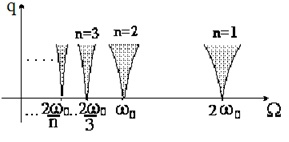
\includegraphics[scale=0.8]{fig2}
\caption{Зоны генерации (заштрихованные области) при параметрическом  \\ возбуждении (без потерь энергии)}
	\end{center}
\end{figure}

\newpage

\subsubsection*{Параметрическое возбуждение при диссипации энергии}

При отсутствии потерь в колебательной системе (т.е. в отсутствие затухания),  параметрический резонанс возникает при любой, сколь угодно малой глубине накачки (рис. 2). Но в   реальных системах с затуханием собственных колебаний из-за потерь энергии (например, на трение)  резонанс может возникнуть только при достижении  некоторой пороговой глубины накачки, когда мощность накачки  начнет превосходить рассеиваемую мощность.  При этом существенно изменяется форма зон параметрического  возбуждения (рис.3)

\begin{figure}[h!]
	\begin{center}
	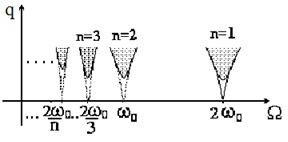
\includegraphics[scale=0.8]{fig3}
\caption{Зоны возбуждения при диссипации энергии}
	\end{center}
\end{figure}

\subsubsection*{Квадрупольный масс-анализатор}

На рис.4. изображен квадрупольный конденсатор (вид с торца стержней). Будем считать электрическое поле не зависящим от продольной координаты z.

\begin{figure}[h!]
	\begin{center}
	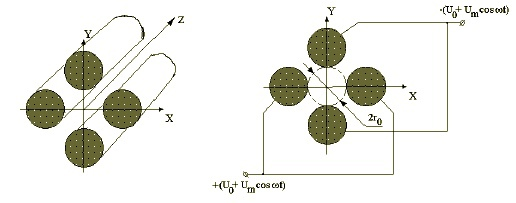
\includegraphics[scale=0.5]{fig4}
\caption{Зоны возбуждения при диссипации энергии}
	\end{center}
\end{figure}

Тогда  электрический потенциал в поле квадрупольного конденсатора будет иметь вид:  $\phi=U_0\frac{x^2-y^2}{2R_0^2}$, где   – разность потенциалов, приложенная между двумя параллельными стержнями; $R_0$ – расстояние от оси системы до оси любого стержня. Напряженность  электрического поля при известном потенциале дается выражением  ,  т.е.: $ E_x=-\frac{\partial\phi}{\partial x}=-\frac{U_0x}{R_0^2};{\ }\mathrm{\ \ \ \ \ \ \ }E_y=-\frac{\partial\phi}{\partial y}=-\frac{U_0y}{R_0^2};{\ }\mathrm{\ \ \ \ \ \ \ }E_z=-\frac{\partial\phi}{\partial z}=0    $       (ф.12)
Если ионы исследуемого вещества направить в конденсатор вдоль оси z с некоторой  произвольно направленной начальной скоростью, то их движение будет описываться уравнениями II закона Ньютона:$
m\frac{d^2x}{dt^2}=-\frac{eU_0x}{R_0^2};{\ }\mathrm{\ \ \ \ \ \ \ \ \ \ \ }m\frac{d^2y}{dt^2}=\frac{eU_0y}{R_0^2};{\ }\mathrm{\ \ \ \ \ \ \ \ \ \ \ }m\frac{d^2z}{dt^2}=0     $                                    (ф.13)
Если теперь к стержням квадрупольного конденсатора кроме постоянного напряжения  приложить  $U_0$  еще и переменное напряжение с амплитудой   и  с частотой (накачки) $\Omega$ так, что суммарное напряжение равно  ,  то уравнения движения принимают   вид:
$\frac{d^2x}{dt^2}+\left(\frac{eU_0}{mR_0^2}+\frac{eU_\Omega}{mR_0^2}cos{\Omega}t\right)х=0;   \frac{d^2y}{dt^2}-\left(\frac{eU_0}{mR_0^2}+\frac{eU_{\Omega}}{ mR_0^2}cos\Omega t \right) у=0;\frac{d^2z}{dt^2}=0$   (ф.14)
Введем  безразмерные величины: $\omega_0^2=\frac{eU_0}{mR_0^2};     q=\frac{U_\Omega}{U_0};                    $ (ф.15)
тогда уравнения движения (3)  принимают вид уравнений Матье:
   $ \frac{d^2x}{dt^2}+\omega_0^2\left(1+qcos{\Omega}t\right)х=0;        \frac{d^2y}{dt^2}-\omega_0^2(1+qcos\Omega t)у=0;\frac{d^2z}{dt^2}=0                         $ (ф.16)
                 Как и в любой системе с параметрической накачкой  резонанс имеет место при  таких значениях  и q, которые лежат в зонах неустойчивости.  

\newpage

\section*{Ход работы}

Включим вакуумную часть установки и произведем откачку системы до вакуума не хуже, чем $10^-4$ Торр

В представлении в виде диаграммы каждому интервалу масс длиной 1 а.е.м. отвечает одна диаграммная линия, в аналоговом режиме такому интервалу отвечает 10 точек. По горизонтальной оси указана масса ионов в а. е. м. (атомных единицах массы).

\subsubsection*{Измерение масс-спектров остаточных газов}

Запустим программу <<EasyView>>, включим накал катода масс-сектрометра и будем снимать показания программы каждые 5 минут. Полученные масс-спектры представлены на рисунках 5 - 7.


\begin{figure}[h!]
	\begin{center}
	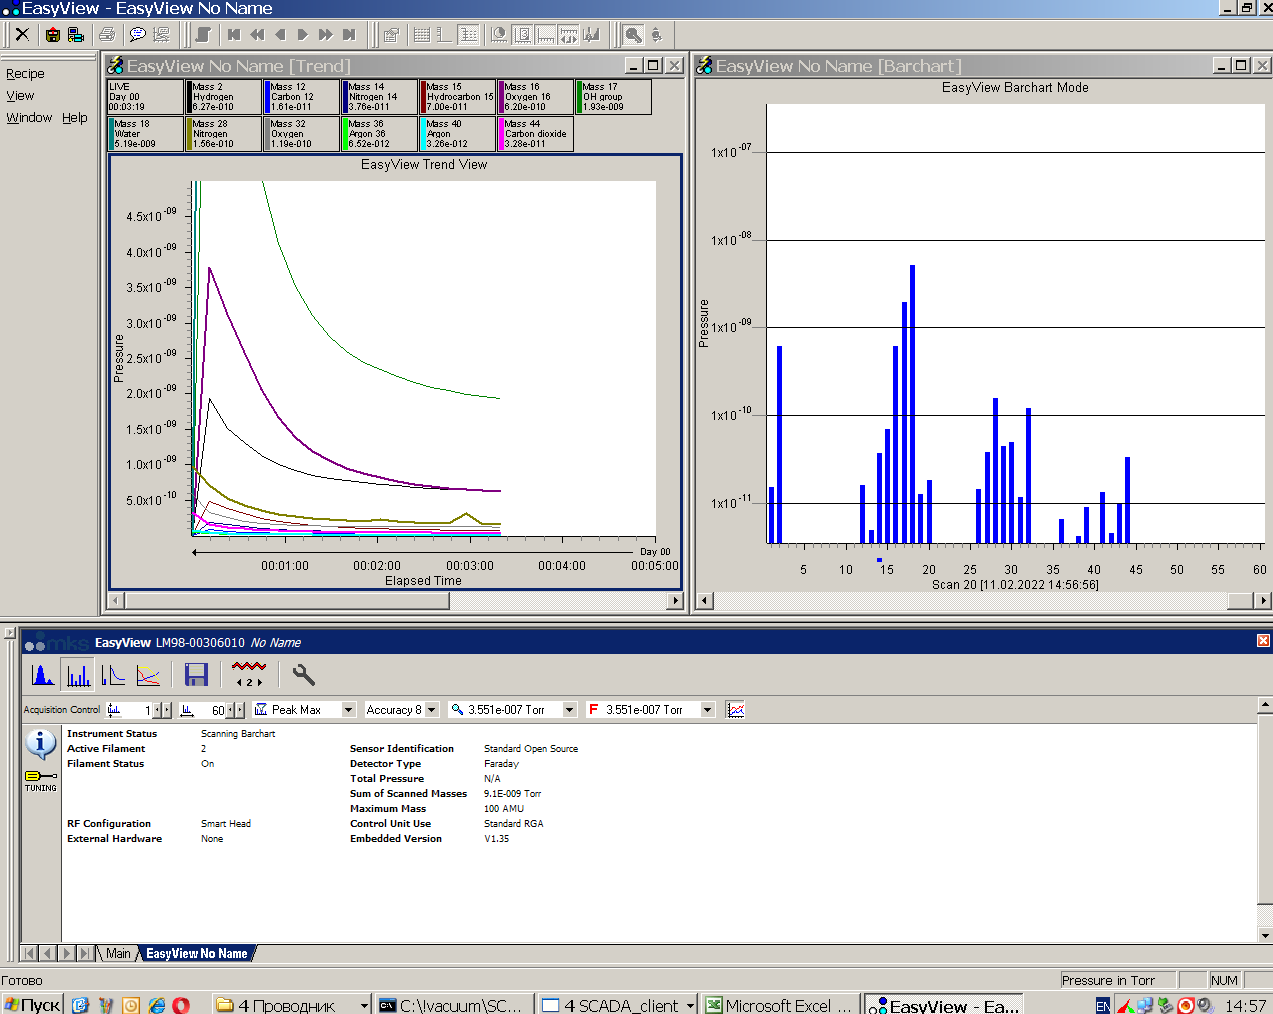
\includegraphics[scale=0.4]{graph1}
	\caption{Первое измерение}
	\end{center}
\end{figure}
\newpage
\begin{figure}[h!]
	\begin{center}
	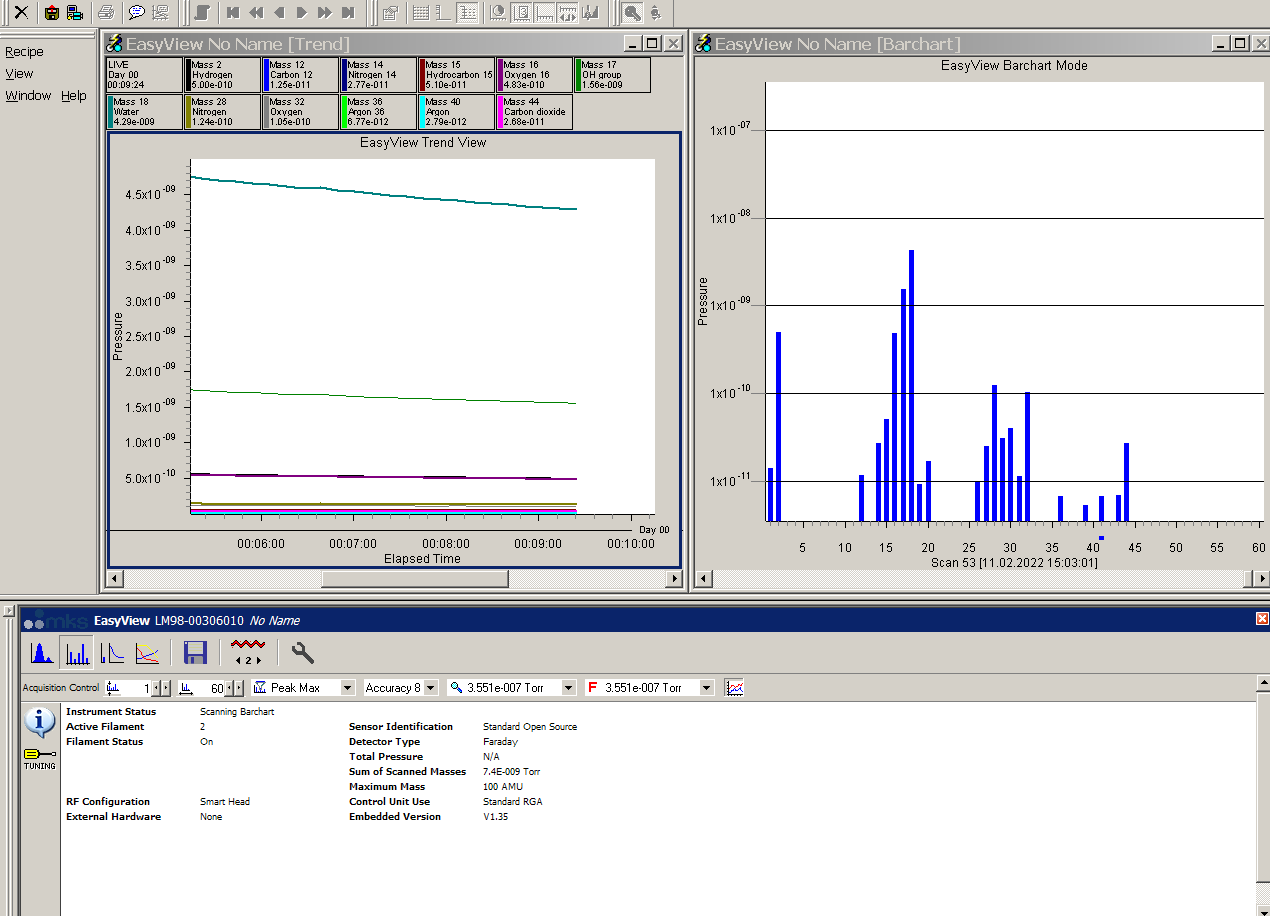
\includegraphics[scale=0.4]{graph2}
	\caption{Второе измерение}
	\end{center}
\end{figure}

\begin{figure}[h!!]
	\begin{center}
	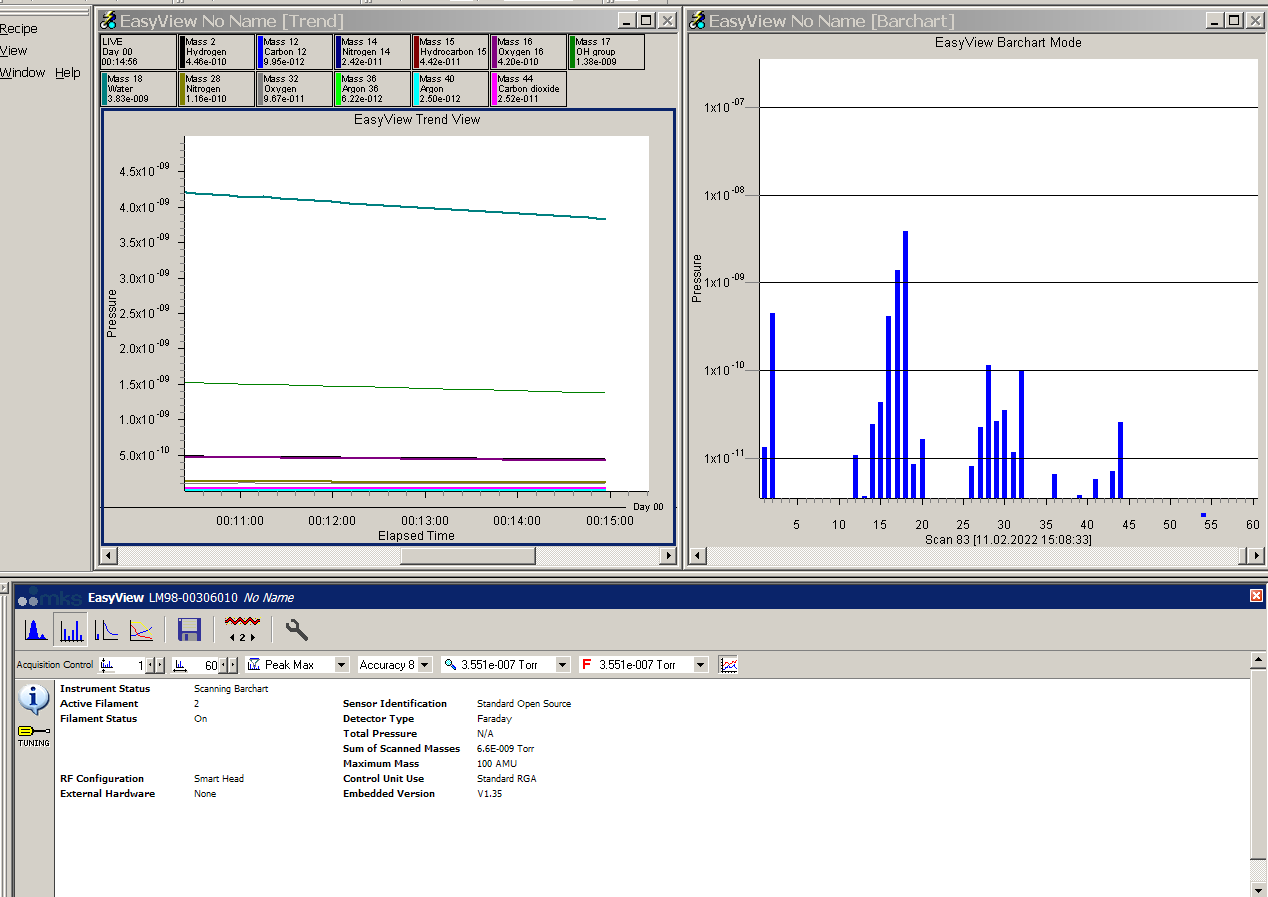
\includegraphics[scale=0.4]{graph3}
	\caption{Третье измерение}
	\end{center}
\end{figure}

\newpage

\begin{figure}[h!]
	\begin{center}
	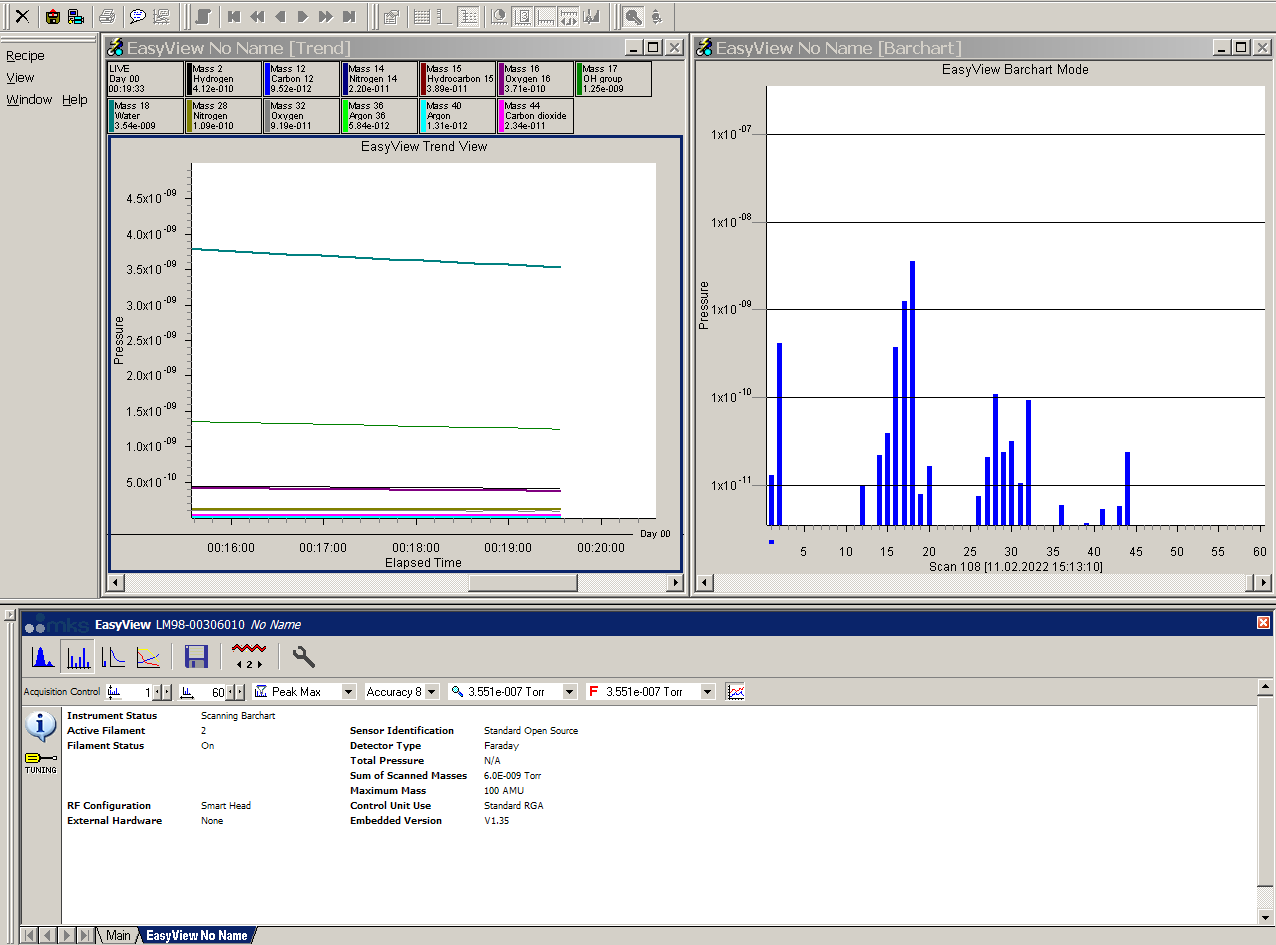
\includegraphics[scale=0.4]{graph4}
	\caption{Четвертое измерение}
	\end{center}
\end{figure}

\subsubsection*{Измерение масс-спектров при напускании газа}

Откроем клапан напускания газа и так же будем снимать показания программы <<EasyView>> каждый 5 минут. Полученные масс-спектры представлены на рисунках 8 - 13.

\begin{figure}[h!]
	\begin{center}
	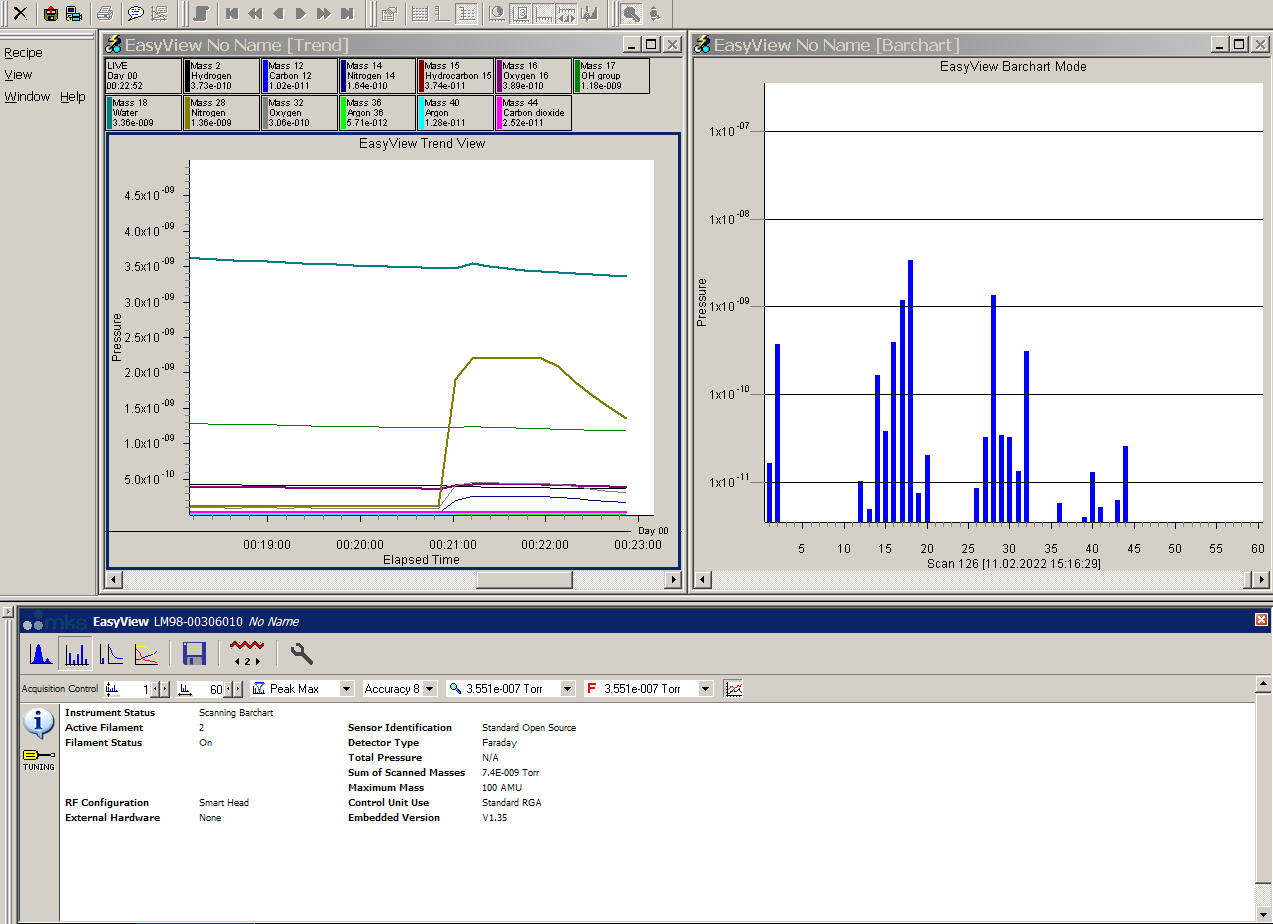
\includegraphics[scale=0.4]{graph5}
	\caption{Первое измерение}
	\end{center}
\end{figure}

\newpage

\begin{figure}[h!]
	\begin{center}
	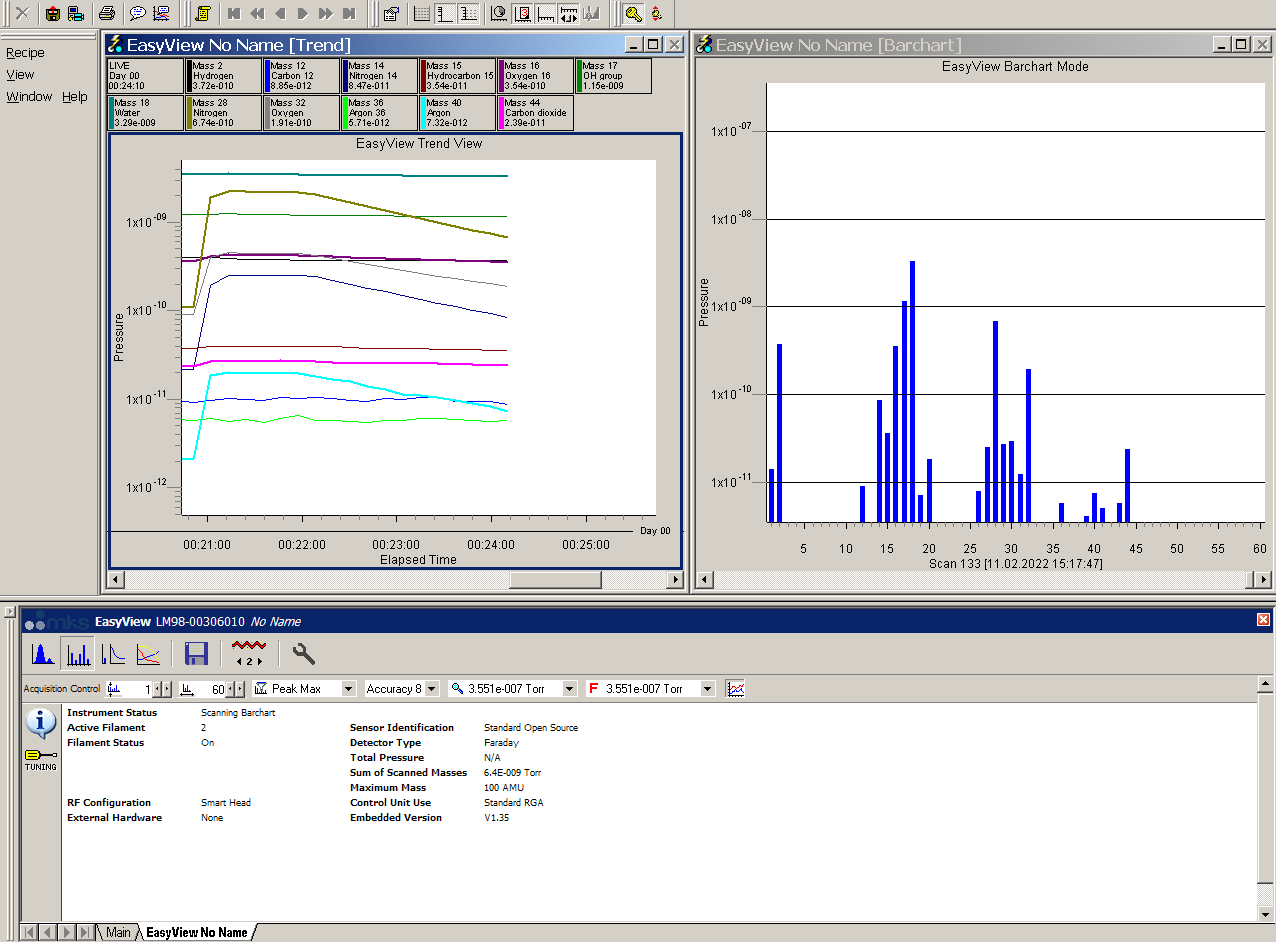
\includegraphics[scale=0.4]{graph6}
	\caption{Второе измерение}
	\end{center}
\end{figure}

\begin{figure}[h!]
	\begin{center}
	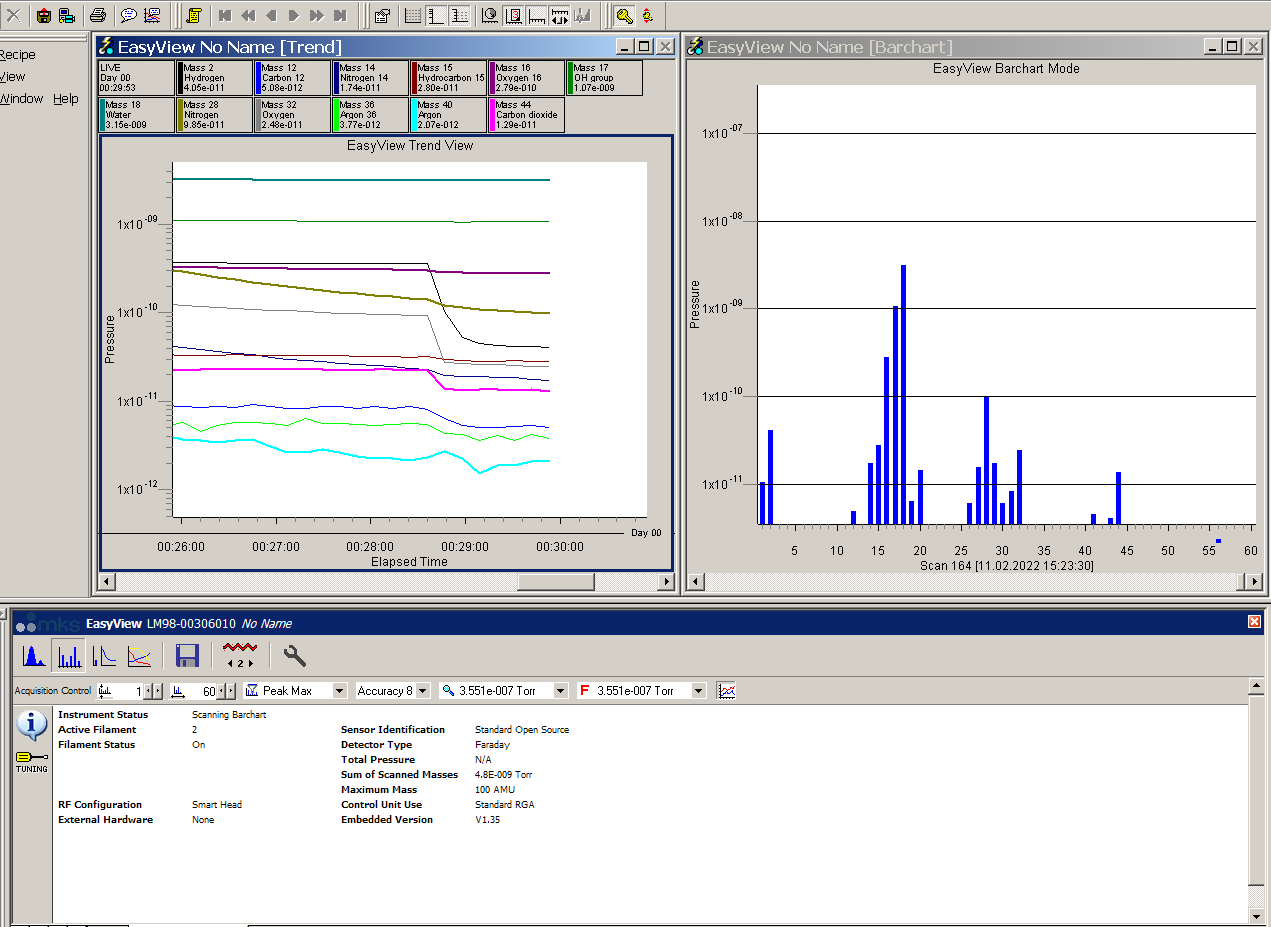
\includegraphics[scale=0.4]{graph7}
	\caption{Третье измерение (выключили ионизационный вакууметр)}
	\end{center}
\end{figure}

\newpage

\begin{figure}[h!]
	\begin{center}
	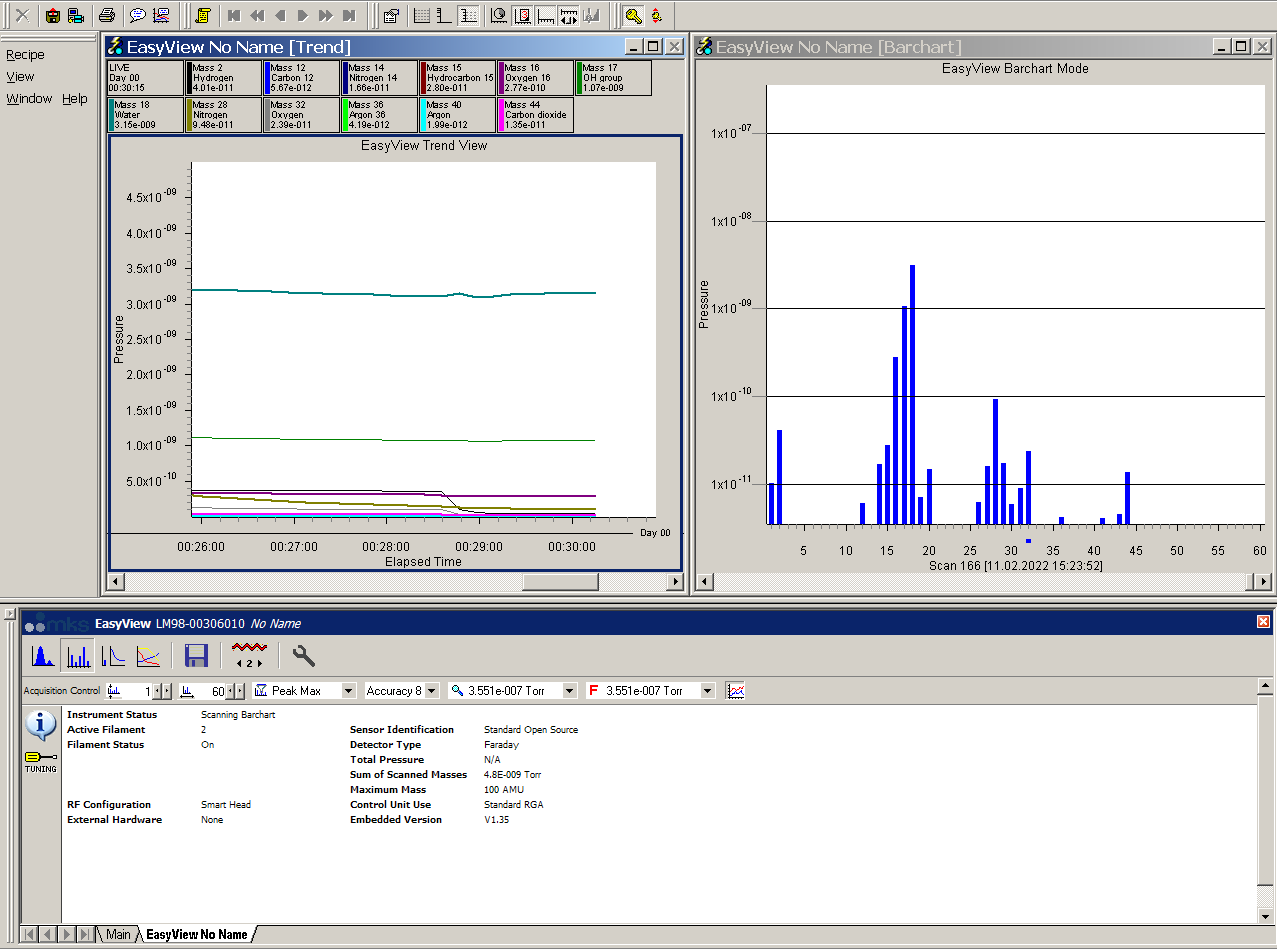
\includegraphics[scale=0.4]{graph8}
	\caption{Четвертое измерение}
	\end{center}
\end{figure}


\section*{Выводы}

1.Ознакомились с методом масс-спектроскопии и принципами работы квадрупольного масс-спектрометра \\
2.Из Рис.5 - Рис.8, что водяные пары составляют б$\acute{о}$льшую часть остаточных газов и, следовательно, их сложнее откачать. \\
3.Был исследован спектр газовой смеси после напускания.
























\end{document}